\chapter{Complejidad temporal}

\index{complejidad temporal}

La eficiencia de los algoritmos es importante en la programación competitiva.
Por lo general, es fácil diseñar un algoritmo
que resuelve el problema lentamente,
pero el verdadero desafío es inventar un
algoritmo rápido.
Si el algoritmo es demasiado lento, obtendrá solo
puntos parciales o ningún punto en absoluto.

La \key{complejidad temporal} de un algoritmo
estima cuánto tiempo utilizará el algoritmo
para alguna entrada.
La idea es representar la eficiencia
como una función cuyo parámetro es el tamaño de la entrada.
Al calcular la complejidad temporal,
podemos averiguar si el algoritmo es lo suficientemente rápido
sin implementarlo.

\section{Reglas de cálculo}

La complejidad temporal de un algoritmo
se denota $O(\cdots)$
donde los tres puntos representan alguna
función.
Por lo general, la variable $n$ denota
el tamaño de la entrada.
Por ejemplo, si la entrada es un conjunto de números,
$n$ será el tamaño del conjunto,
y si la entrada es una cadena,
$n$ será la longitud de la cadena.

\subsubsection*{Bucles}

Una razón común por la que un algoritmo es lento es
que contiene muchos bucles que recorren la entrada.
Cuanto más bucles anidados contenga el algoritmo,
más lento será.
Si hay $k$ bucles anidados,
la complejidad temporal es $O(n^k)$.

Por ejemplo, la complejidad temporal del siguiente código es $O(n)$:
\begin{lstlisting}
for (int i = 1; i <= n; i++) {
    // código
}
\end{lstlisting}

Y la complejidad temporal del siguiente código es $O(n^2)$:
\begin{lstlisting}
for (int i = 1; i <= n; i++) {
    for (int j = 1; j <= n; j++) {
        // código
    }
}
\end{lstlisting}

\subsubsection*{Orden de magnitud}

Una complejidad temporal no nos dice el número exacto
de veces que se ejecuta el código dentro de un bucle,
sino que solo muestra el orden de magnitud.
En los siguientes ejemplos, el código dentro del bucle
se ejecuta $3n$, $n+5$ y $\lceil n/2 \rceil$ veces,
pero la complejidad temporal de cada código es $O(n)$.

\begin{lstlisting}
for (int i = 1; i <= 3*n; i++) {
    // código
}
\end{lstlisting}

\begin{lstlisting}
for (int i = 1; i <= n+5; i++) {
    // código
}
\end{lstlisting}

\begin{lstlisting}
for (int i = 1; i <= n; i += 2) {
    // código
}
\end{lstlisting}

Como otro ejemplo,
la complejidad temporal del siguiente código es $O(n^2)$:

\begin{lstlisting}
for (int i = 1; i <= n; i++) {
    for (int j = i+1; j <= n; j++) {
        // código
    }
}
\end{lstlisting}

\subsubsection*{Fases}

Si el algoritmo consta de fases consecutivas,
la complejidad temporal total es la mayor
complejidad temporal de una sola fase.
La razón de esto es que la fase más lenta
suele ser el cuello de botella del código.

Por ejemplo, el siguiente código consta
de tres fases con complejidades temporales
$O(n)$, $O(n^2)$ y $O(n)$.
Por lo tanto, la complejidad temporal total es $O(n^2)$.

\begin{lstlisting}
for (int i = 1; i <= n; i++) {
    // código
}
for (int i = 1; i <= n; i++) {
    for (int j = 1; j <= n; j++) {
        // código
    }
}
for (int i = 1; i <= n; i++) {
    // código
}
\end{lstlisting}

\subsubsection*{Varias variables}

A veces la complejidad temporal depende de
varios factores.
En este caso, la fórmula de complejidad temporal
contiene varias variables.

Por ejemplo, la complejidad temporal del
siguiente código es $O(nm)$:

\begin{lstlisting}
for (int i = 1; i <= n; i++) {
    for (int j = 1; j <= m; j++) {
        // código
    }
}
\end{lstlisting}

\subsubsection*{Recursión}

La complejidad temporal de una función recursiva
depende del número de veces que se llama a la función
y la complejidad temporal de una sola llamada.
La complejidad temporal total es el producto de
estos valores.

Por ejemplo, considere la siguiente función:
\begin{lstlisting}
void f(int n) {
    if (n == 1) return;
    f(n-1);
}
\end{lstlisting}
La llamada $\texttt{f}(n)$ provoca $n$ llamadas a la función,
y la complejidad temporal de cada llamada es $O(1)$.
Por lo tanto, la complejidad temporal total es $O(n)$.

Como otro ejemplo, considere la siguiente función:
\begin{lstlisting}
void g(int n) {
    if (n == 1) return;
    g(n-1);
    g(n-1);
}
\end{lstlisting}
En este caso, cada llamada a la función genera dos otras
llamadas, excepto para $n=1$.
Veamos qué sucede cuando se llama a $g$
con el parámetro $n$.
La siguiente tabla muestra las llamadas a la función
producidas por esta única llamada:
\begin{center}
\begin{tabular}{rr}
llamada a la función & número de llamadas \\
\hline
$g(n)$ & 1 \\
$g(n-1)$ & 2 \\
$g(n-2)$ & 4 \\
$\cdots$ & $\cdots$ \\
$g(1)$ & $2^{n-1}$ \\
\end{tabular}
\end{center}
Basándonos en esto, la complejidad temporal es
\[1+2+4+\cdots+2^{n-1} = 2^n-1 = O(2^n).\]

\section{Clases de complejidad}

\index{clases de complejidad}

La siguiente lista contiene complejidades temporales comunes
de los algoritmos:

\begin{description}
\item[$O(1)$]
\index{algoritmo de tiempo constante}
El tiempo de ejecución de un algoritmo \key{de tiempo constante}
no depende del tamaño de la entrada.
Un algoritmo típico de tiempo constante es una fórmula directa
que calcula la respuesta.

\item[$O(\log n)$]
\index{algoritmo logarítmico}
Un algoritmo \key{logarítmico} a menudo reduce a la mitad
el tamaño de la entrada en cada paso.
El tiempo de ejecución de dicho algoritmo
es logarítmico, porque
$\log_2 n$ es igual al número de veces
que $n$ debe dividirse por 2 para obtener 1.

\item[$O(\sqrt n)$]
Un \key{algoritmo de raíz cuadrada} es más lento que
$O(\log n)$ pero más rápido que $O(n)$.
Una propiedad especial de las raíces cuadradas es que
$\sqrt n = n/\sqrt n$, por lo que la raíz cuadrada $\sqrt n$ se encuentra,
en cierto sentido, en el medio de la entrada.

\item[$O(n)$]
\index{algoritmo lineal}
Un algoritmo \key{lineal} recorre la entrada
un número constante de veces.
Esta es a menudo la mejor complejidad temporal posible,
ya que generalmente es necesario acceder a cada
elemento de entrada al menos una vez antes de
informar la respuesta.

\item[$O(n \log n)$]
Esta complejidad temporal a menudo indica que el
algoritmo ordena la entrada,
porque la complejidad temporal de los algoritmos de ordenamiento
eficientes es $O(n \log n)$.
Otra posibilidad es que el algoritmo
utilice una estructura de datos en la que cada operación
tarda $O(\log n)$ en tiempo.

\item[$O(n^2)$]
\index{algoritmo cuadrático}
Un algoritmo \key{cuadrático} a menudo contiene
dos bucles anidados.
Es posible recorrer todos los pares de
los elementos de entrada en tiempo $O(n^2)$.

\item[$O(n^3)$]
\index{algoritmo cúbico}
Un algoritmo \key{cúbico} a menudo contiene
tres bucles anidados.
Es posible recorrer todos los tríos de
los elementos de entrada en tiempo $O(n^3)$.

\item[$O(2^n)$]
Esta complejidad temporal a menudo indica que
el algoritmo itera a través de todos
los subconjuntos de los elementos de entrada.
Por ejemplo, los subconjuntos de $\{1,2,3\}$ son
$\emptyset$, $\{1\}$, $\{2\}$, $\{3\}$, $\{1,2\}$,
$\{1,3\}$, $\{2,3\}$ y $\{1,2,3\}$.

\item[$O(n!)$]
Esta complejidad temporal a menudo indica que
el algoritmo itera a través de todas
las permutaciones de los elementos de entrada.
Por ejemplo, las permutaciones de $\{1,2,3\}$ son
$(1,2,3)$, $(1,3,2)$, $(2,1,3)$, $(2,3,1)$,
$(3,1,2)$ y $(3,2,1)$.

\end{description}

\index{algoritmo polinomial}
Un algoritmo es \key{polinomial}
si su complejidad temporal es como máximo $O(n^k)$
donde $k$ es una constante.
Todas las complejidades temporales anteriores excepto
$O(2^n)$ y $O(n!)$ son polinomiales.
En la práctica, la constante $k$ suele ser pequeña,
y por lo tanto, una complejidad temporal polinomial
significa aproximadamente que el algoritmo es \emph{eficiente}.

\index{problema NP-difícil}

La mayoría de los algoritmos en este libro son polinomiales.
Sin embargo, hay muchos problemas importantes para los cuales
no se conoce ningún algoritmo polinomial, es decir,
nadie sabe cómo resolverlos de manera eficiente.
Los problemas \key{NP-difíciles} son un conjunto importante
de problemas, para los cuales no se conoce ningún algoritmo
polinomial\footnote{Un libro clásico sobre el tema es
\emph{Computers and Intractability: A Guide to the Theory
of NP-Completeness} de M. R. Garey y D. S. Johnson \cite{gar79}.}.

\section{Estimación de la eficiencia}

Al calcular la complejidad temporal de un algoritmo,
es posible verificar, antes de
implementar el algoritmo, que es
suficientemente eficiente para el problema.
El punto de partida para las estimaciones es el hecho de que
una computadora moderna puede realizar varios cientos de
millones de operaciones en un segundo.

Por ejemplo, supongamos que el límite de tiempo para
un problema es de un segundo y el tamaño de entrada es $n=10^5$.
Si la complejidad temporal es $O(n^2)$,
el algoritmo realizará aproximadamente $(10^5)^2=10^{10}$ operaciones.
Esto debería tomar al menos unas decenas de segundos,
por lo que el algoritmo parece ser demasiado lento para resolver el problema.

Por otro lado, dado el tamaño de entrada,
podemos intentar \emph{adivinar}
la complejidad temporal requerida del algoritmo
que resuelve el problema.
La siguiente tabla contiene algunas estimaciones útiles
suponiendo un límite de tiempo de un segundo.

\begin{center}
\begin{tabular}{ll}
tamaño de entrada & complejidad temporal requerida \\
\hline
$n \le 10$ & $O(n!)$ \\
$n \le 20$ & $O(2^n)$ \\
$n \le 500$ & $O(n^3)$ \\
$n \le 5000$ & $O(n^2)$ \\
$n \le 10^6$ & $O(n \log n)$ o $O(n)$ \\
$n$ es grande & $O(1)$ o $O(\log n)$ \\
\end{tabular}
\end{center}

Por ejemplo, si el tamaño de entrada es $n=10^5$,
probablemente se espera que la complejidad
temporal del algoritmo sea $O(n)$ o $O(n \log n)$.
Esta información facilita el diseño del algoritmo,
porque descarta enfoques que generarían
un algoritmo con una peor complejidad temporal.

\index{factor constante}

Aun así, es importante recordar que una
complejidad temporal es solo una estimación de la eficiencia,
porque oculta los \emph{factores constantes}.
Por ejemplo, un algoritmo que se ejecuta en tiempo $O(n)$
puede realizar $n/2$ o $5n$ operaciones.
Esto tiene un efecto importante en el tiempo de ejecución
real del algoritmo.

\section{Suma máxima de subarreglo}

\index{suma máxima de subarreglo}

A menudo hay varios algoritmos posibles
para resolver un problema de manera que sus
complejidades temporales sean diferentes.
Esta sección analiza un problema clásico que
tiene una solución directa de $O(n^3)$.
Sin embargo, al diseñar un algoritmo mejor, es
posible resolver el problema en tiempo $O(n^2)$
e incluso en tiempo $O(n)$.

Dado un arreglo de $n$ números,
nuestra tarea es calcular la
\key{suma máxima de subarreglo}, es decir,
la suma más grande posible de
una secuencia de valores consecutivos
en el arreglo\footnote{El libro de J. Bentley \emph{Programming Pearls} \cite{ben86} hizo popular el problema.}.
El problema es interesante cuando puede haber
valores negativos en el arreglo.
Por ejemplo, en el arreglo
\begin{center}
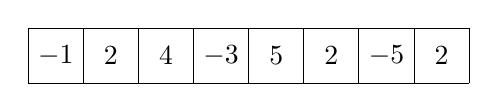
\begin{tikzpicture}[scale=0.7]
\draw (0,0) grid (8,1);

\node at (0.5,0.5) {$-1$};
\node at (1.5,0.5) {$2$};
\node at (2.5,0.5) {$4$};
\node at (3.5,0.5) {$-3$};
\node at (4.5,0.5) {$5$};
\node at (5.5,0.5) {$2$};
\node at (6.5,0.5) {$-5$};
\node at (7.5,0.5) {$2$};
\end{tikzpicture}
\end{center}
\begin{samepage}
the following subarray produces the maximum sum $10$:
\begin{center}
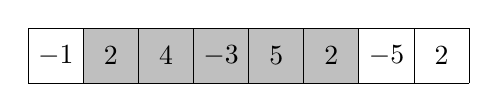
\begin{tikzpicture}[scale=0.7]
\fill[color=lightgray] (1,0) rectangle (6,1);
\draw (0,0) grid (8,1);

\node at (0.5,0.5) {$-1$};
\node at (1.5,0.5) {$2$};
\node at (2.5,0.5) {$4$};
\node at (3.5,0.5) {$-3$};
\node at (4.5,0.5) {$5$};
\node at (5.5,0.5) {$2$};
\node at (6.5,0.5) {$-5$};
\node at (7.5,0.5) {$2$};
\end{tikzpicture}
\end{center}
\end{samepage}

We assume that an empty subarray is allowed,
so the maximum subarray sum is always at least $0$.

\subsubsection{Algorithm 1}

A straightforward way to solve the problem
is to go through all possible subarrays,
calculate the sum of values in each subarray and maintain
the maximum sum.
The following code implements this algorithm:

\begin{lstlisting}
int best = 0;
for (int a = 0; a < n; a++) {
    for (int b = a; b < n; b++) {
        int sum = 0;
        for (int k = a; k <= b; k++) {
            sum += array[k];
        }
        best = max(best,sum);
    }
}
cout << best << "\n";
\end{lstlisting}

The variables \texttt{a} and \texttt{b} fix the first and
last index of the subarray,
and the sum of values is calculated to the variable \texttt{sum}.
The variable \texttt{best} contains the maximum sum found during the search.

The time complexity of the algorithm is $O(n^3)$,
because it consists of three nested loops 
that go through the input.

\subsubsection{Algorithm 2}

It is easy to make Algorithm 1 more efficient
by removing one loop from it.
This is possible by calculating the sum at the same
time when the right end of the subarray moves.
The result is the following code:

\begin{lstlisting}
int best = 0;
for (int a = 0; a < n; a++) {
    int sum = 0;
    for (int b = a; b < n; b++) {
        sum += array[b];
        best = max(best,sum);
    }
}
cout << best << "\n";
\end{lstlisting}
After this change, the time complexity is $O(n^2)$.

\subsubsection{Algorithm 3}

Surprisingly, it is possible to solve the problem
in $O(n)$ time\footnote{In \cite{ben86}, this linear-time algorithm
is attributed to J. B. Kadane, and the algorithm is sometimes
called \index{Kadane's algorithm} \key{Kadane's algorithm}.}, which means
that just one loop is enough.
The idea is to calculate, for each array position,
the maximum sum of a subarray that ends at that position.
After this, the answer for the problem is the
maximum of those sums.

Consider the subproblem of finding the maximum-sum subarray
that ends at position $k$.
There are two possibilities:
\begin{enumerate}
\item The subarray only contains the element at position $k$.
\item The subarray consists of a subarray that ends
at position $k-1$, followed by the element at position $k$.
\end{enumerate}

In the latter case, since we want to
find a subarray with maximum sum,
the subarray that ends at position $k-1$
should also have the maximum sum.
Thus, we can solve the problem efficiently
by calculating the maximum subarray sum
for each ending position from left to right.

The following code implements the algorithm:
\begin{lstlisting}
int best = 0, sum = 0;
for (int k = 0; k < n; k++) {
    sum = max(array[k],sum+array[k]);
    best = max(best,sum);
}
cout << best << "\n";
\end{lstlisting}

The algorithm only contains one loop
that goes through the input,
so the time complexity is $O(n)$.
This is also the best possible time complexity,
because any algorithm for the problem
has to examine all array elements at least once.

\subsubsection{Efficiency comparison}

It is interesting to study how efficient 
algorithms are in practice.
The following table shows the running times
of the above algorithms for different
values of $n$ on a modern computer.

In each test, the input was generated randomly.
The time needed for reading the input was not
measured.

\begin{center}
\begin{tabular}{rrrr}
array size $n$ & Algorithm 1 & Algorithm 2 & Algorithm 3 \\
\hline
$10^2$ & $0.0$ s & $0.0$ s & $0.0$ s \\
$10^3$ & $0.1$ s & $0.0$ s & $0.0$ s \\
$10^4$ & > $10.0$ s & $0.1$ s & $0.0$ s \\
$10^5$ & > $10.0$ s & $5.3$ s & $0.0$ s \\
$10^6$ & > $10.0$ s & > $10.0$ s & $0.0$ s \\
$10^7$ & > $10.0$ s & > $10.0$ s & $0.0$ s \\
\end{tabular}
\end{center}

The comparison shows that all algorithms
are efficient when the input size is small,
but larger inputs bring out remarkable
differences in the running times of the algorithms.
Algorithm 1 becomes slow
when $n=10^4$, and Algorithm 2
becomes slow when $n=10^5$.
Only Algorithm 3 is able to process
even the largest inputs instantly.
